\mychapter{\textsc{Fundamentação Teórica}}{chp:fundamentacao}
\lhead{\textsc{Fundamentação Teórica}}


\lettrine{A} fundamentação deste trabalho encontra-se respaldado na teoria dos grafos, na análise de redes sociais e medidas de centralidade de redes complexas. 

\section{\textbf{Teoria dos Grafos}}\label{sec:grafos} 

Em teoria de grafos, temos que um grafo é o conjunto de $G = (\bm V,\bm E)$ ($G$ = Grafos, $V$ = Vértices e $E$ = Arestas), onde $V$ é um conjunto não vazio de objetos denominados vértices (ou nós) e $E$ é um subconjunto de pares não ordenados de $V$. Neste entendimento temos que grafos pode serem caracterizados no prisma de algumas propriedades, como por exemplo o comportamento da ligação das arestas pode ser classificado como não direcional ou direcional, onde cada aresta $\Vec E$ de $\Vec G = (\bm V,\bm \Vec E)$ possui um sentido ou orientação definido por um par ordenado $(\bm x_{1}, \bm x_{2})$, sendo $x_{1}$ o ponto inicial e $x_{2}$ o ponto final da aresta em questão.

O estudo de redes complexas é um tema  que abrange diversas áreas de conhecimento, tais como a ciência da computação, matemática, física, biologia e sociologia. 
O termo ``redes complexas'' refere-se a um grafo que apresenta uma estrutura topográfica não trivial, composto por um conjunto de vértices (nós) que são interligados por meio de arestas \citep{barabasi2003everything}. 
O estudo de redes na forma de grafos é um dos pilares da matemática discreta e teve início em 1735, quando Euler propôs uma solução para o problema das pontes de Königsberg, originando a teoria dos grafos.

Redes de coautoria se caracteriza por ligação não direcional, ou seja, que independe de quem seja o ponto de origem para o destino da ligação, pois devemos para a proposta deste trabalho, considerar que se uma instituição publicou um artigo em coautoria com outra instituição, a recíproca é verdadeira e não há distinção de qual tem propriedades valoradas, como a iniciativa ou mesmo o grau de participação do coautor na publicação em tela.

As figuras abaixo representam a plotagem de grafos apresentando a visão da abordagem de coautorias intra-regional conforme a Figura~\ref{grafo1}, e coautorias inter-regional vide Figura~\ref{grafo2}, onde $S$ é a representação da região da instituição, $X$ os autores (vértices ou nós) e as arestas/ligações representam a relação de coautoria entre eles.


\begin{figure}[H]
\centering
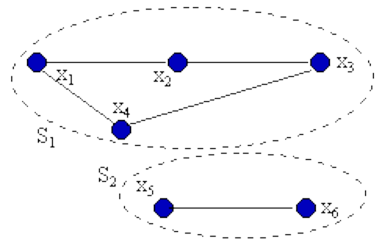
\includegraphics[scale=0.8]{Imagens/intra-grafo.pdf}
\caption{Grafo com representação de Rede de Coautoria intra grupos}
\label{grafo1}
\end{figure}

\begin{figure}[H]
\centering
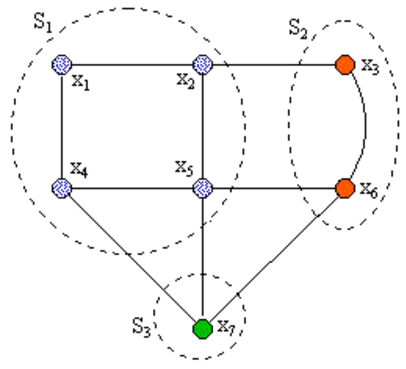
\includegraphics[scale=0.8]{Imagens/inter-grafo.pdf}
\caption{Grafo com representação de Rede de Coautoria inter grupos}
\label{grafo2}
\end{figure}

\section{\textbf{Análise de Redes Sociais}}\label{sec:redes_sociais}

Conforme \citep{Silva2006}, a análise de redes sociais interessa a pesquisadores de vários campos do conhecimento que, na tentativa de compreender o seu impacto sobre a vida social, deram origem a diversas metodologias de análise que têm como base as relações entre os indivíduos, em uma estrutura em forma de redes.

A análise de redes sociais (ARS ou SNA, da expressão em inglês \textit{Social Network Analysis)} é uma abordagem oriunda da sociologia, da psicologia social e da antropologia. \citep{freeman1996some,wasserman1994social}. ARS não é algo recente, há estudos, como o trabalho de \citep{otte2002social} que buscou desde a década de 1970, análises de redes de informação, de pesquisadores e de citações, como também de redes de coautoria.

 Redes de couatoria utiliza-se da análise de redes sociais embasada nas propriedades e aplicações de redes complexas, a qual vemos a seguir.


\begin{figure}[H]
\centering
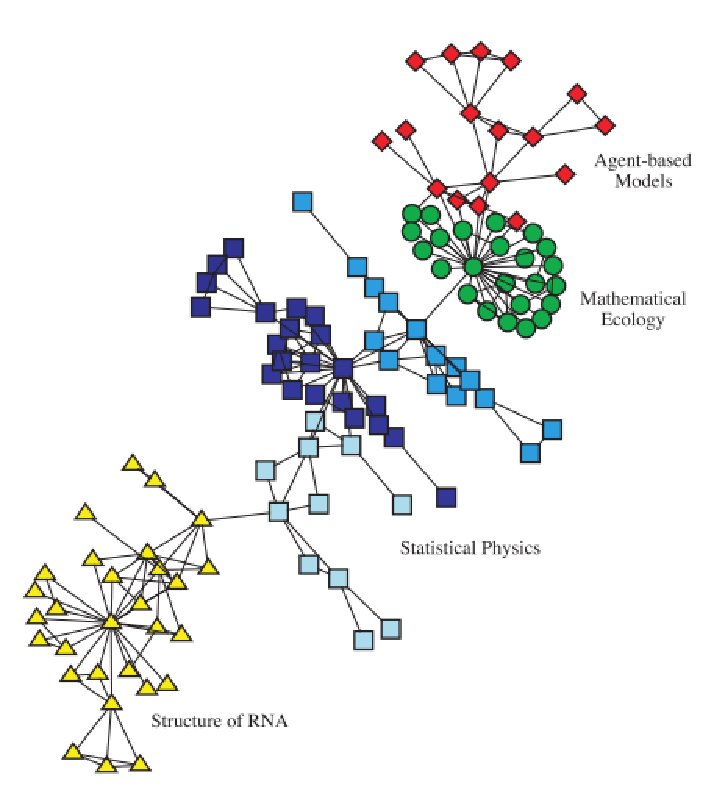
\includegraphics[scale=0.7]{Imagens/rede-newman.pdf}
\caption{Pequena Rede de Coautoria de Newman}
\label{rede1}
\end{figure}

\section{\textbf{Redes Complexas}}\label{sec:redes_complexas}

No contexto da teoria de redes complexas, uma rede corresponde a um grafo, que se representa por um conjunto de nós ligados por arestas, que em conjunto formam uma rede.  Esta rede ou grafo, permite representar relações com fundamento das propriedades dos vários tipos de grafos e como são constituídos, ou seja, como se agrupam os seus nós e são ligadas suas arestas %\cite{mendes2005fisica}.

As propriedades de redes complexas às quais utilizaremos nesse trabalho se encontram definidas a seguir.

\noindent \textbf{Definição 2.3.1} (Grau de um nó). O número de vértices adjacentes a um determinado vértice $x_i$ chama-se de grau de $x_i$. Em um grafo direcionado $\Vec G = (\bm V,\bm \Vec E)$, diferenciamos o grau de saída (output) do grau de entrada (input):

\begin{equation}
k^{out}_{x_{i}}(\Vec{G}) = \sum_{x_j \in V : x_j \neq x_i}^{} A[x_i,x_j]
\label{eq:grauOutput}
\end{equation}

\begin{equation}
k^{in}_{x_{i}}(\Vec{G}) = \sum_{x_j \in V : x_j \neq x_i}^{} A[x_j,x_i]
\label{eq:grauInput}
\end{equation}

Desse modo, chamamos de grau de $x_i$: 

\begin{equation}
k_{x_i}(\Vec{G}) = k^{out}_{x_{i}}(\Vec{G}) + k^{in}_{x_{i}}(\Vec{G})
\label{eq:grau}
\end{equation}

\noindent \textbf{Definição 2.3.2} (Centralidade de um nó - \textit{Degree centrality}). Definida como o número de ligações incidentes de um vértice, esta medida nos informa qual a probabilidade de um vértice receber alguma informação da rede. Logo, a centralidade de um vértice $v$ de um grafo $G = (\bm V,\bm E)$ é dada por:

\begin{equation}
    C_D(\bm v) = deg(\bm v)
\end{equation}

Uma vez que a direção das arestas podem influenciar o cálculo, em redes direcionadas existem duas medidas distintas de centralidade de grau: indegree, que corresponde ao número de ligações direcionadas para o nó e outdegree, que consiste no número de ligações que o nó encaminha para os demais vértices da rede. 

\noindent \textbf{Definição 2.3.3} (Intermediação - \textit{Betweenness centrality}). Trata-se de uma medida de centralidade de um grafo baseada em caminhos mínimos. A intermediação de um nó $v$ é dada do seguinte modo: 

\begin{equation}
    g(\bm v) = \sum_{s \neq t \neq v} \frac{\sigma_{st}(v)}{\sigma_{st}}
\end{equation}

Onde $\sigma_{st}$ é o número total de caminhos mínimos do nó $s$ para o nó $t$ e $\sigma_{st}(v)$ é o número de caminhos mínimos de $s$ para $t$ que utilizam o nó $v$ como intermediário.

 A intermediação também pode ser normalizada, sem perda de precisão, dividindo seu resultado pelo número de pares de nós não incluindo $v$, de maneira que $g(\bm v) \in [0,1]$. Tal medida é vista como mais poderosa que apenas a conectividade, uma vez que fornece uma informação mais global sobre a rede em questão.

\noindent \textbf{Definição 2.3.4} (Proximidade - \textit{Closeness Centrality}). Em um grafo conectado, a proximidade de um nó é uma medida de centralidade calculada pela inversa da soma do comprimento dos caminhos mínimos entre um dado nó $v$ e todos os demais nós do grafo. Desse modo, quanto mais central for o nó, mais próximo dos demais esse se encontrará. Sua fórmula é definida como:

\begin{equation}
    C(\bm v) = \frac{1}{\sum_{\forall u \in V, u\neq v}d_G(u,v)}
\end{equation}

Onde, $d(u,v)$ é a distância do caminho mínimo entre $u$ e $v$.

Usualmente, na literatura costuma-se usar sua versão normalizada, dada não mais pela soma de seus caminhos mínimos e sim pela média destes, como visto a seguir:

\begin{equation}
    C(\bm v) = \frac{N - 1}{\sum_{\forall u \in V, u\neq v}d_G(u,v)}
\end{equation}

Onde, $N$ é o número de nós do grafo, ou seja, $N = |V|$. Para grafos extremamente grandes a diferença $- 1$ torna-se irrelevante, podendo ser descartada.

%\noindent \textbf{Definição 2.3.5} (Diâmetro). É definido como a excentricidade máxima entre dois nós. A excentricidade de um nó $x_i$ é definida como a distância máxima de $x_i$ a todos os outros nós do grafo $G$.

\noindent \textbf{Definição 2.3.5} (Coeficiente de agregação ou aglomeração - \textit{clustering coefficient}). Trata-se do número de ligações entre os vizinhos mais próximos de um nó.

\noindent \textbf{Definição 2.3.6} (Redes estáticas/dinâmicas). Uma rede é estática quando não há variação do número de nós e, é dinâmica, quando é possível modelar o seu crescimento pela análise da variação da sua estrutura ao longo do tempo.

Os estudos das medidas de centralidade de redes foram evoluindo ao longo do tempo; centralidade, proximidade e intermediação é apontada por \citep{freeman1996some}, como medidas essenciais aos estudos e análises de redes. 

A figura abaixo ilustra a topologogia das medidas de centralidade: a) \textit{degree centrality}; b) \textit{closeness centrality} e c) \textit{betweeness centrality}. Com elas podemos perceber por meio dos vértices de cor vermelha a disposição dos mesmos na topologia da rede, e seus respectivos posicionamaentos, nos levando a compreender o tipo da sua centralidade e seu papel na rede.

\begin{figure}[H]
\centering
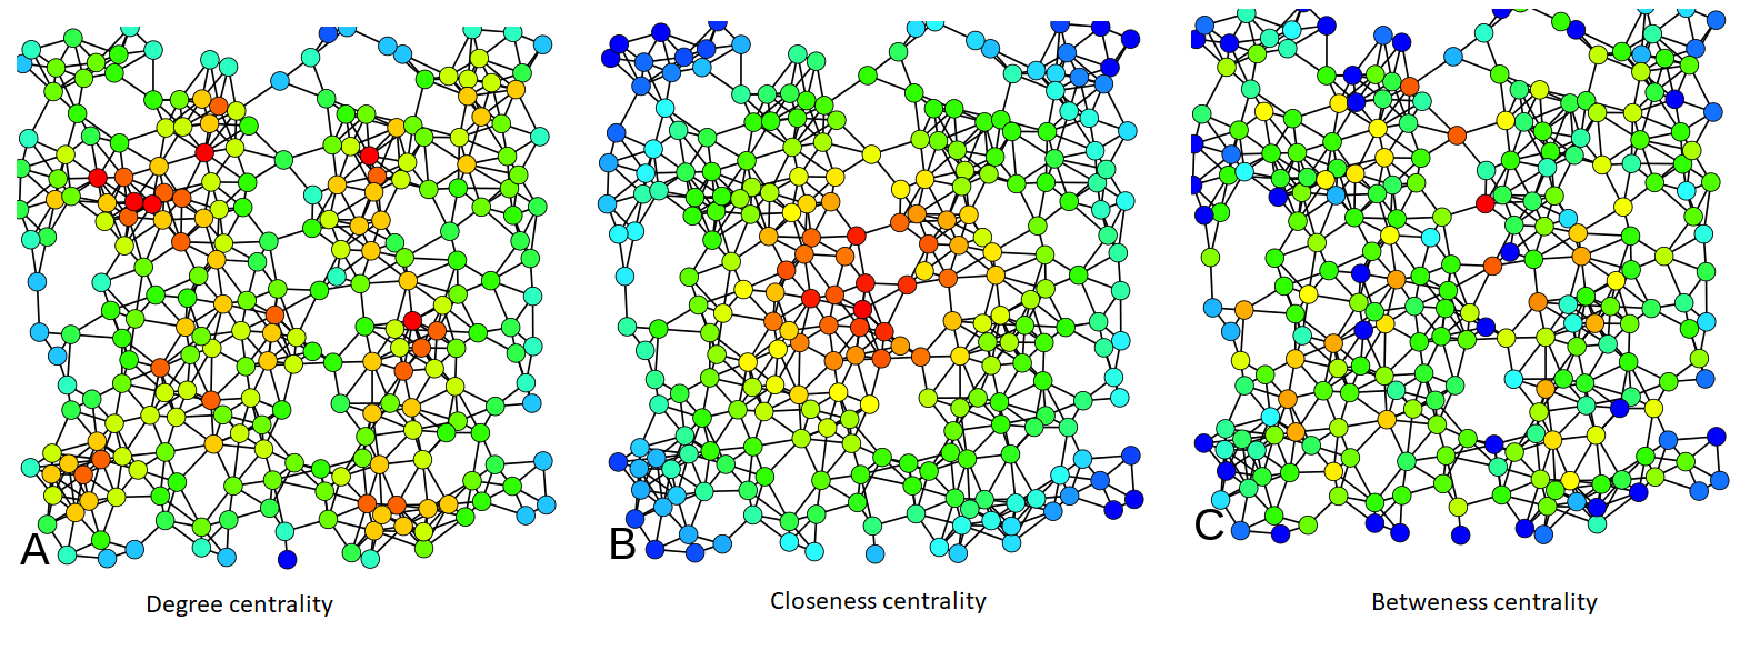
\includegraphics[scale=0.5]{Imagens/Centrality.pdf}
\caption{Redes com ilustração das medidas de centralidade (Fonte: Claudio Rocchini - Adaptado)}
\label{centrality}
\end{figure}

\section{\textbf{Colaboração Científica}}\label{sec:colab} 

Colaboração científica pode ser definida como interação que ocorre dentro de um contexto social entre dois ou mais cientistas, que facilita a partilha de significado e conclusão de tarefas em relação a um objetivo mútuo, compartilhado e organizado. Os cientistas que colaboram também podem trazer metas individuais adicionais para uma colaboração. \citep{Sonnenwald}

Ainda, segundo a autora, a colaboração ocorre dentro do contexto social da ciência, que inclui elementos como a revisão por pares, sistemas de prêmios, paradigmas científicos, políticas de ciência nacionais e internacionais, bem como normas implícitas ao campo disciplinar das instituições de pesquisa e/ou universidades. 

Conforme \citep{Newman2004}, há algum tempo se percebe que a coautoria de artigos em periódicos acadêmicos fornece uma janela sobre padrões de colaboração dentro da comunidade acadêmica. 

Para \citep{Sonnenwald}, estudos da colaboração científica está aumentando, por possuir o potencial de auxiliar a resolução de problemas científicos complexos e promover agendas políticas, econômicas e sociais. 

\resumocap{Neste Capítulo, explanamos os conhecimentos e fundamentações teóricas necessárias para este trabalho. No Capítulo seguinte é apresentada a metodologia utilizada para o desenvolvimento deste.}

